\section{Framework}
This secion explains the development methodology and organisation of this
project.
\subsection{Software development methodology}
\label{sec:dev_method}
As this project has been very time restricted, the development needed to be as
efficient as possible. The project group therefore had to find a model that
utilized the available manpower in the best possible way. Considering the small
size of the project group, big and complex development models would add too much
bureaucracy to coordinate the project and has thus been out of the question. A
lightweight and efficient development model was preferred, so the group chose to
go for an agile \cite{AGILE} development model (figure \ref{fig:development_model}) structured
into development cycles. This way, each group member could take an active part in the project and
all members could feel a sense of ownership.

\begin{figure}[ht!]
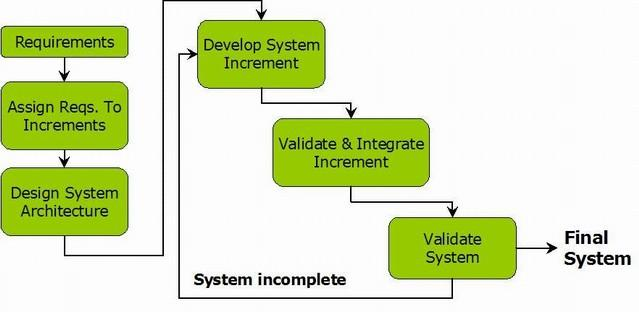
\includegraphics[width=130mm]{./img/development_model.png}
\caption{Agile development model}
\label{fig:development_model}
\end{figure}

By developing iterative and incrementally, the group combined the best from
both the agile development world and from the very well defined waterfall
approach \cite{waterfall}. Feedback from Avdeling BKI and the project mentor has
been very important in the course of the project, in addition to having a
structured and reasonable way of actually doing changes to the plan while the
project was running. At the same time the group was able to maintain the
overall plan within cycles, so that it was possible to work individually, while
still being well coordinated.

To be able to develop all the modules of the project within the timeframe, each
development cycle consisted of multiple modules or functionality developed in
parallel. This allowed for good utilization of time and personnel. The start of
each cycle consisted of a meeting where the goals for the cycle were defined and
individual tasks that we needed to get done were identified. This process bears
similarity to the start of a sprint in the development model Scrum \cite{scrum}.
During the development part of the cycle, the group worked individually on the
tasks that were defined in the planning phase. Regular meetings and cooperative
programming within the group ensured that everyone pulled the project in the
same direction. At the end of each cycle a working set of software was ready,
which ideally complied with all the goals set in the start of each cycle.
Meetings with Avdeling BKI were held between each cycle to present the progress,
and to let them influence the direction of the project.

When all the development cycles were completed, final assurances were made that
everything worked as intended and that all modules coexisted in harmony. This
part of the development also consisted of some hands-on testing by Avdeling BKI
and performance testing.

\subsection{Schedule}
This project had a fairly comprehensive initial phase for mapping
and designing of the system. The group spent the better part of the first two
weeks figuring out how to implement the system. After the two weeks and before
the start of the development, a ``project decision meeting" was held with
Avdeling BKI to get feedback on the design and confirm that the system was
modelled correctly for their needs.

After this, the implementation phase commenced, which consisted of development
cycles as described above in section \ref{sec:dev_method}. This phase was devided into
five parts: four development cycles and a final cleanup/testing cycle. All the
development cycles lasted two weeks, aside from the last development cycle and the cleanup/testing
cycle, which lasted one week each. During these cycles the group conducted
meetings with both the project mentor and Avdeling BKI every two weeks, timed so
that these meetings took place on alternating weeks. This ensured continual
feedback and advice throughout the development process.

After the development phase, focus was shifted from the software to the project
report, and the group spent the final 5-6 weeks working on the report. The group
benefitted from the work performed during the first weeks of the project which
could go almost directly into the report.

\subsection{Project Organization}
The organisation of the project shifted throughout the project, reflecting
the fact that the project had multiple phases. During the first few weeks
the group spent most of the time together in a group room, cooperating in
forming the design and discussing various solutions. Once most things had been
worked out and the implementation phase began, there was more room and need to
work individually to produce code. In this period, the group gathered
together a few times a week to syncronize the progress and plan the next course
of action. Throughout the project, most decisions have been made either by
confering with the client or achieving consensus within the group. 
